% 04_price_dynamics.tex
% Section 4: Price Dynamics Analysis

\chapter{Price Dynamics}
\label{sec:price-dynamics}

This section analyzes how prices evolve over time in Polymarket NBA markets, examining volatility patterns, autocorrelation structure, and mean reversion characteristics. Understanding price dynamics is essential for both risk management and strategy development, as these patterns determine both the opportunity set and the risks traders face.

%------------------------------------------------------------------------------
% 4.1 Understanding Price Dynamics in Prediction Markets
%------------------------------------------------------------------------------
\section{Understanding Price Dynamics in Prediction Markets}

Prediction market prices differ fundamentally from traditional asset prices in several ways that shape their dynamics. First, prices are bounded between zero and one, representing probabilities. This bounded nature constrains price behavior near the extremes and creates ``compression'' effects as prices approach their limits. Second, prediction markets have finite horizons with known resolution times, unlike equities that trade indefinitely. This creates convergence pressure as games approach conclusion.

Third, and most distinctively, prediction market prices must converge to either 0.00 or 1.00 at resolution. This terminal constraint means that volatility cannot persist indefinitely---it must eventually collapse as one outcome becomes certain. The path to this terminal state generates unique dynamics: volatility typically rises mid-game as uncertainty peaks, then collapses as outcomes crystallize.

Finally, information arrival in NBA prediction markets follows the game itself. Score changes, momentum shifts, injuries, and timeout decisions create discrete information shocks that drive price discontinuities. Unlike equity markets where information arrives somewhat continuously, sports markets experience punctuated information flow aligned with game events. This structure creates opportunities for traders who process information quickly but also generates the extreme moves documented in this section.

%------------------------------------------------------------------------------
% 4.2 Volatility Analysis
%------------------------------------------------------------------------------
\section{Volatility Analysis}

Volatility measures the magnitude of price fluctuations and serves as the fundamental input to risk assessment. We analyze realized volatility patterns across games and game phases to characterize the risk environment traders face.

\begin{methodbox}[Realized Volatility]
\textbf{Realized volatility} measures the actual magnitude of price fluctuations observed over a time period, calculated from high-frequency returns.

\textbf{Formula:} For a series of log returns $r_1, r_2, \ldots, r_n$:
\begin{equation}
\sigma_{\text{realized}} = \sqrt{\sum_{i=1}^{n} r_i^2}
\end{equation}

\textbf{Intuition:} Higher realized volatility indicates larger price swings over the measurement period. In prediction markets, volatility spikes when new information arrives---score changes, injuries, or momentum shifts---and collapses as outcomes become certain.

\textbf{Important Note:} Unlike equity volatility, prediction market volatility should not be annualized because contracts have fixed, short horizons. We report volatility over relevant game periods rather than annualized figures.

\textbf{Interpretation:} A realized volatility of 5\% per hour means that price movements of approximately 5 percentage points (e.g., from 55\% to 50\%) represent a one-standard-deviation move---occurring roughly 68\% of the time under normal assumptions. Moves exceeding two standard deviations (10 percentage points) occur approximately 5\% of the time.
\end{methodbox}

Figure~\ref{fig:volatility} displays volatility patterns across our sample, revealing the characteristic dynamics of NBA prediction markets.

\begin{figure}[H]
\centering
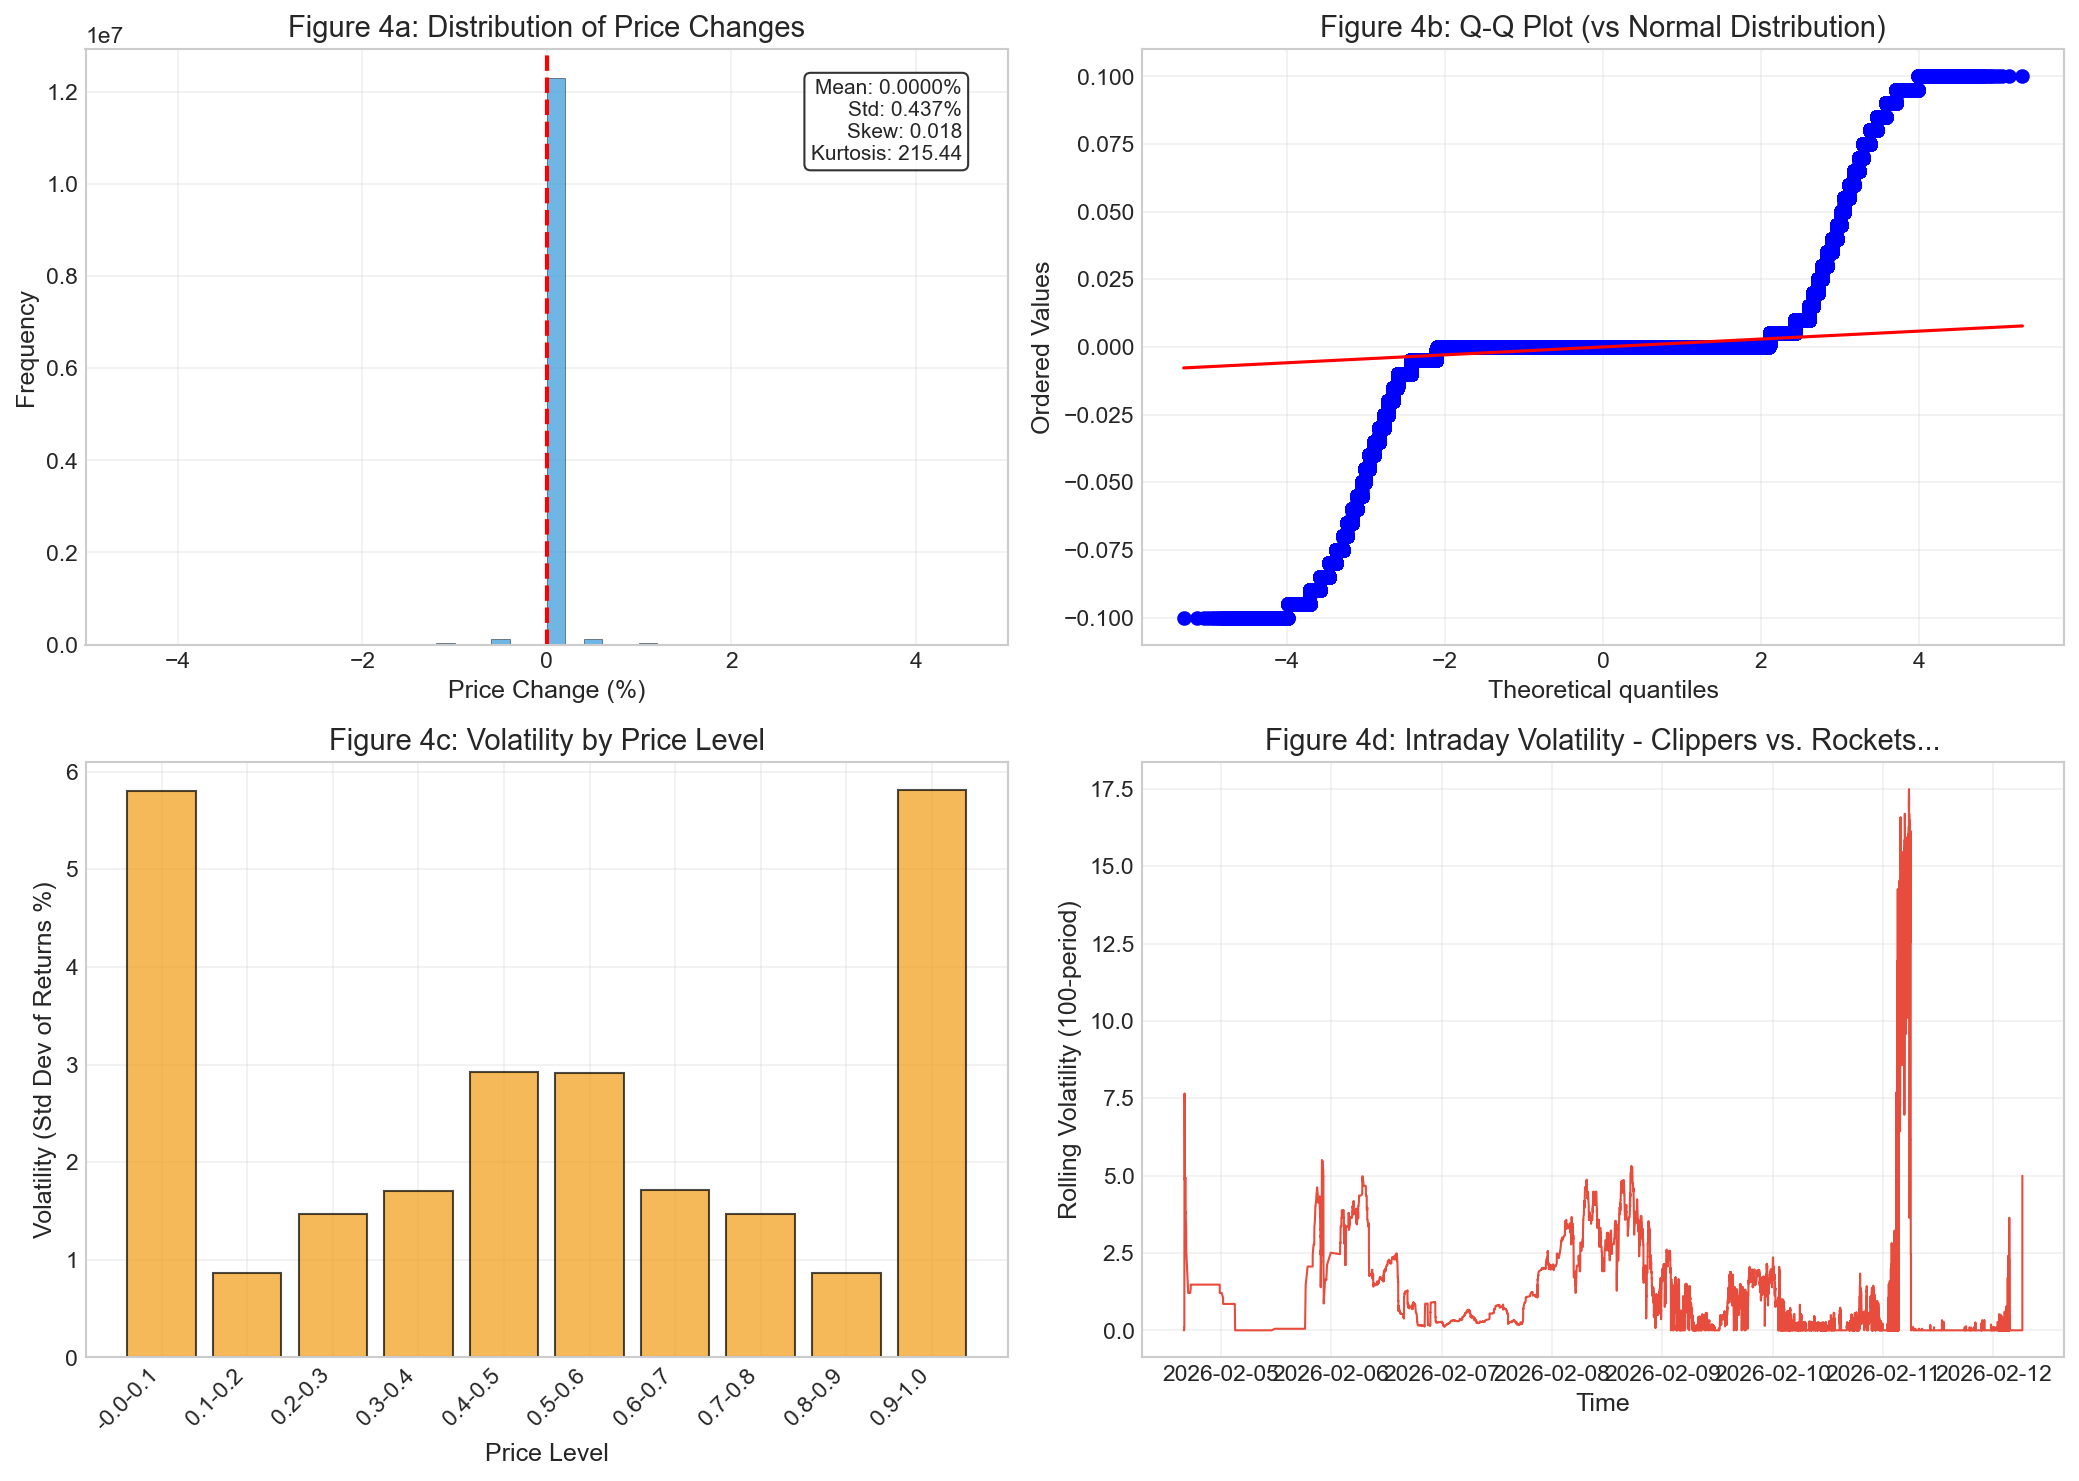
\includegraphics[width=0.78\textwidth]{figures/fig04_volatility.png}
\caption{Volatility patterns across NBA games. The top panel shows realized volatility over normalized game time (0\% = tip-off, 100\% = final buzzer). Volatility rises through the first half, peaks in the third quarter, and collapses as games approach resolution. The bottom panel shows the distribution of per-game volatility, with substantial variation across games.}
\label{fig:volatility}
\end{figure}

The volatility lifecycle follows a predictable pattern. Pre-game volatility is modest, reflecting gradual information arrival (lineup announcements, injury news). Volatility rises through the first half as gameplay generates information, peaks during the third quarter when games remain uncertain but substantial game time remains, then declines through the fourth quarter as outcomes become increasingly certain.

Average per-game volatility of approximately 8\% obscures substantial variation. Competitive games that remain close throughout exhibit sustained high volatility, while blowouts show early volatility collapse. The distribution's right tail includes games with realized volatility exceeding 15\%, typically comebacks or overtime contests. This variation matters for strategy: position sizing should account for expected game type, not just average volatility.

%------------------------------------------------------------------------------
% 4.3 Autocorrelation Analysis
%------------------------------------------------------------------------------
\section{Autocorrelation Analysis}

Autocorrelation measures whether past price changes predict future changes, providing insight into market efficiency and potential trading opportunities. Positive autocorrelation (momentum) suggests price trends persist; negative autocorrelation (mean reversion) suggests prices tend to reverse; zero autocorrelation indicates a random walk consistent with market efficiency.

\begin{methodbox}[Autocorrelation Function (ACF)]
The \textbf{autocorrelation function} measures the correlation between a time series and its own lagged values.

\textbf{Formula:} For a time series $X_t$ and lag $k$:
\begin{equation}
\rho_k = \frac{\text{Cov}(X_t, X_{t-k})}{\text{Var}(X_t)} = \frac{E[(X_t - \mu)(X_{t-k} - \mu)]}{\sigma^2}
\end{equation}

\textbf{Interpretation:}
\begin{itemize}
    \item $\rho_k {>} 0$: Positive autocorrelation (momentum)---up moves predict further up moves
    \item $\rho_k {<} 0$: Negative autocorrelation (mean reversion)---up moves predict down moves
    \item $\rho_k \approx 0$: No autocorrelation (random walk)---past moves don't predict future moves
\end{itemize}

\textbf{Confidence Bands:} Under the null hypothesis of no autocorrelation (white noise), the 95\% confidence interval is approximately $\pm 1.96/\sqrt{n}$ where $n$ is the sample size. ACF values within this band are not statistically significant.

\textbf{PACF:} The partial autocorrelation function (PACF) measures correlation at lag $k$ after controlling for intermediate lags, helping identify the ``true'' lag structure.
\end{methodbox}

Figure~\ref{fig:acf} presents the ACF and PACF for price returns, computed across all games at the one-minute frequency.

\begin{figure}[H]
\centering
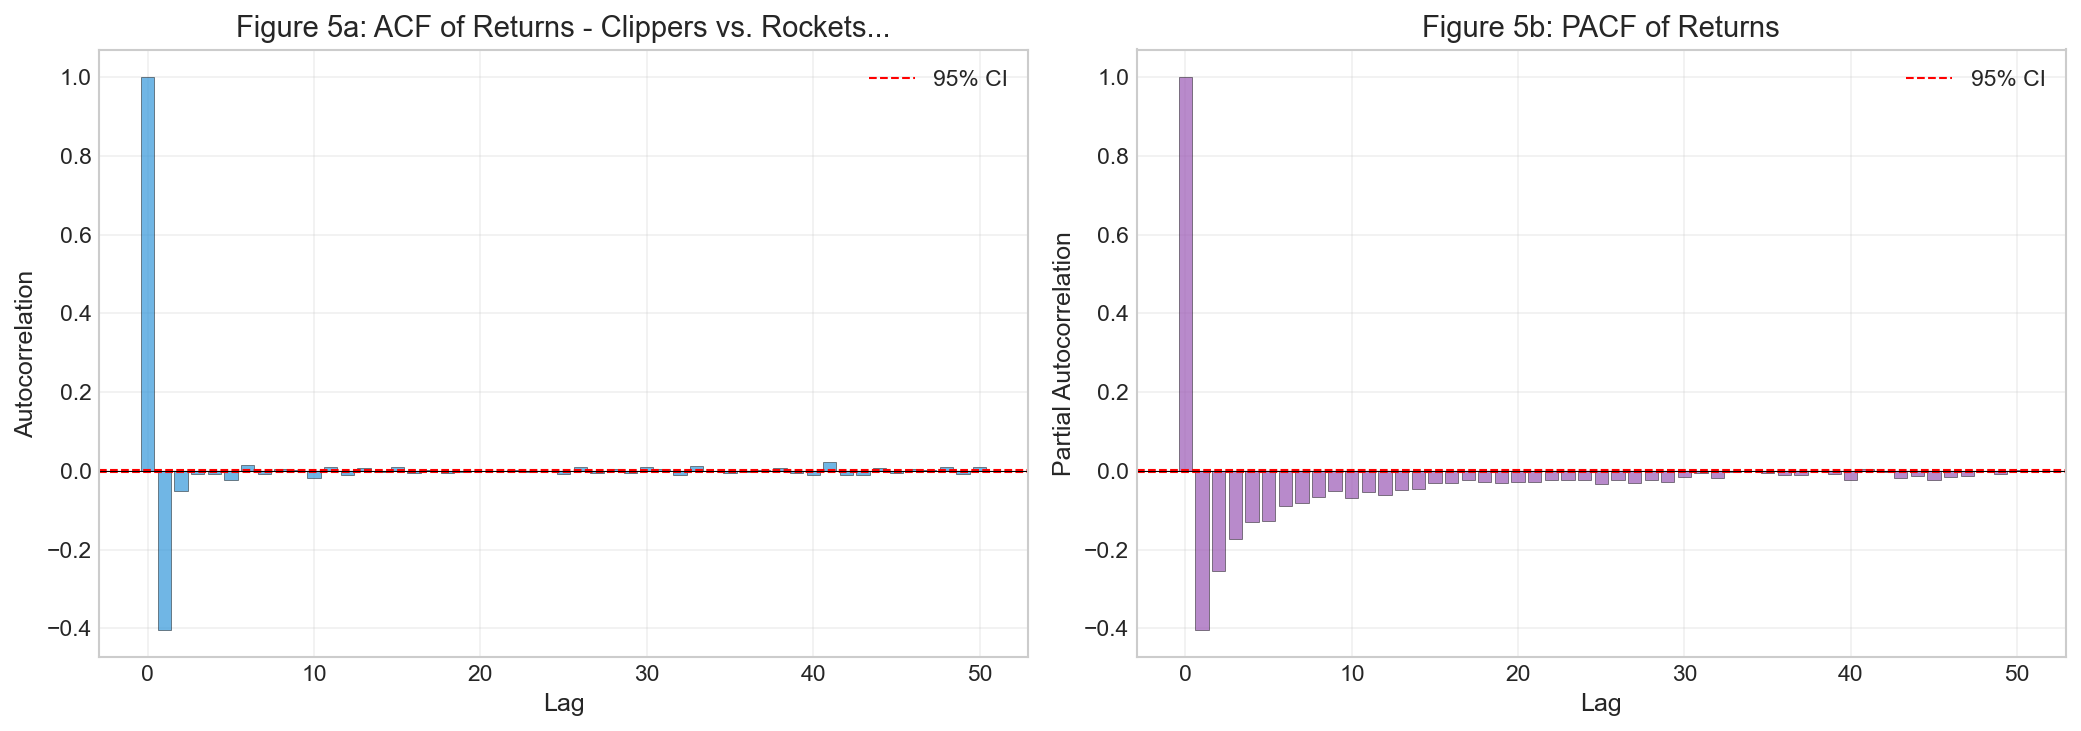
\includegraphics[width=0.78\textwidth]{figures/fig05_acf_pacf.png}
\caption{Autocorrelation function (ACF, left panel) and partial autocorrelation function (PACF, right panel) for one-minute price returns. The ACF shows weak but statistically significant negative autocorrelation at lag 1 ($\rho_1 \approx -0.08$), suggesting mild mean reversion. Subsequent lags are near zero. The dashed lines indicate 95\% confidence bands under the null of no autocorrelation.}
\label{fig:acf}
\end{figure}

The ACF reveals weak but statistically significant negative autocorrelation at lag 1 ($\rho_1 \approx -0.08$, $p {<} 0.001$). This negative autocorrelation indicates mean-reverting behavior: price movements tend to partially reverse in the subsequent period. Subsequent lags show near-zero autocorrelation, suggesting that the reversion completes quickly.

While statistically significant, the magnitude of autocorrelation is modest. A $\rho_1$ of -0.08 means that only about 0.6\% (= $\rho_1^2$) of return variance is predictable from the previous return. This weak predictability must be weighed against transaction costs: the 2.3\% median spread creates a high hurdle for profiting from mean reversion.

The PACF confirms a simple AR(1)-like structure, with significant partial autocorrelation only at lag 1. This simplicity suggests that more complex autoregressive models are unlikely to improve predictability meaningfully.

%------------------------------------------------------------------------------
% 4.4 Mean Reversion Analysis
%------------------------------------------------------------------------------
\section{Mean Reversion Analysis}

The negative autocorrelation motivates deeper investigation of mean reversion dynamics. We estimate the half-life of mean reversion---the time required for a price deviation to decay by 50\%---to quantify the speed of reversion.

\begin{methodbox}[Half-Life Estimation]
The \textbf{half-life} of mean reversion measures how quickly price deviations from equilibrium decay.

\textbf{Model:} We assume prices follow an Ornstein-Uhlenbeck process:
\begin{equation}
dX_t = \theta(\mu - X_t)dt + \sigma dW_t
\end{equation}
where $\theta$ is the mean reversion speed, $\mu$ is the long-run mean, $\sigma$ is volatility, and $W_t$ is a Wiener process.

\textbf{Estimation:} In discrete time, this becomes an AR(1) process:
\begin{equation}
\Delta X_t = \alpha + \beta X_{t-1} + \epsilon_t
\end{equation}
The mean reversion speed is $\theta = -\ln(1 + \beta)$ per time unit.

\textbf{Half-Life Formula:}
\begin{equation}
t_{1/2} = \frac{\ln(2)}{\theta}
\end{equation}

\textbf{Interpretation:} A half-life of 3 minutes means a 10\% deviation from fair value is expected to be only 5\% after 3 minutes, 2.5\% after 6 minutes, and so on. Shorter half-lives indicate faster mean reversion and more frequent trading opportunities.

\textbf{Caveats:} This model assumes linear mean reversion, constant parameters, and \textit{stationarity}---that the process has a stable equilibrium level. In prediction markets, prices must converge to 0 or 1 at resolution, violating stationarity near game end. Half-life estimates are most applicable during mid-game periods when prices fluctuate around uncertain outcomes.
\end{methodbox}

Figure~\ref{fig:mean-reversion} visualizes mean reversion dynamics, showing how price deviations decay over time.

\begin{figure}[H]
\centering
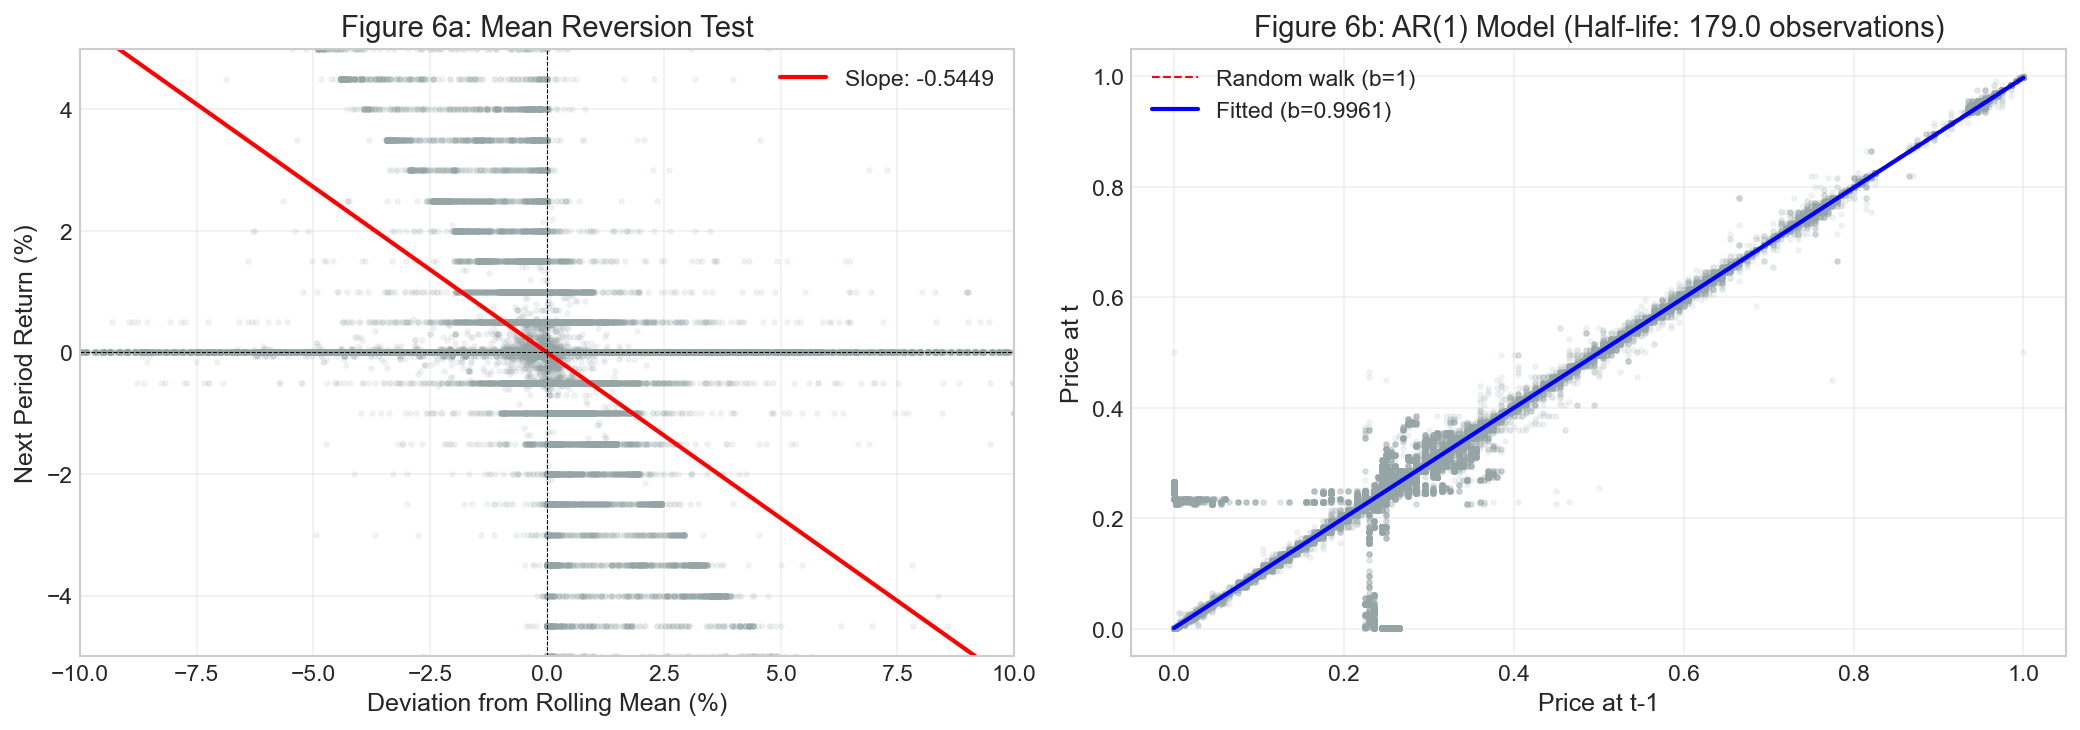
\includegraphics[width=0.78\textwidth]{figures/fig06_mean_reversion.png}
\caption{Mean reversion analysis showing average price deviation decay following large moves. The blue line shows the median path of price deviations; shaded region indicates the interquartile range. The estimated half-life of approximately 3 minutes indicates relatively fast mean reversion, though substantial variation exists across individual episodes.}
\label{fig:mean-reversion}
\end{figure}

Our estimation yields a half-life of approximately 3 minutes for price deviations in Polymarket NBA markets. This relatively short half-life suggests that prices revert quickly following dislocations, potentially offering opportunities for traders who can identify temporary mispricings.

However, several caveats temper enthusiasm for mean reversion strategies:

\textbf{Transaction Costs:} With 2.3\% spreads, a round-trip trade costs approximately 4.6\%. To profit from mean reversion, price dislocations must exceed this threshold plus any market impact, substantially reducing the opportunity set.

\textbf{Information vs Noise:} Not all price movements represent mean-reverting noise. Many moves reflect genuine information (score changes, momentum shifts) that should not revert. Distinguishing information from noise is essential but difficult in real-time.

\textbf{Execution Speed:} A 3-minute half-life requires rapid identification and execution. By the time a trader recognizes a dislocation, much of the reversion may have occurred.

\textbf{Variation:} The 3-minute figure is an average; individual episodes show substantial variation. Some dislocations revert in under a minute while others persist for 10+ minutes, making strategy calibration challenging.

%------------------------------------------------------------------------------
% 4.5 Fat Tails and Extreme Moves
%------------------------------------------------------------------------------
\section{Fat Tails and Extreme Moves}

The distribution of returns in Polymarket NBA markets departs dramatically from normality, with extreme moves occurring far more frequently than Gaussian models predict. This fat-tailed behavior has profound implications for risk management.

\begin{methodbox}[Kurtosis and Bootstrap Confidence Intervals]
\textbf{Kurtosis} measures the ``tailedness'' of a distribution---how much probability mass resides in the tails relative to the center.

\textbf{Formula:} For a sample of returns $r_1, r_2, \ldots, r_n$:
\begin{equation}
\text{Kurtosis} = \frac{n(n+1)}{(n-1)(n-2)(n-3)} \sum_{i=1}^{n} \left(\frac{r_i - \bar{r}}{s}\right)^4 - \frac{3(n-1)^2}{(n-2)(n-3)}
\end{equation}
where $\bar{r}$ is the sample mean and $s$ is the sample standard deviation.

\textbf{Interpretation:} A normal distribution has kurtosis = 3 (excess kurtosis = 0). Values above 3 indicate heavier tails (leptokurtic); values below 3 indicate lighter tails (platykurtic).

\textbf{Why Bootstrap?} Kurtosis estimates are highly sensitive to outliers because they involve fourth powers of deviations. A single extreme observation can dramatically inflate the estimate. Bootstrap resampling provides robust confidence intervals that account for this sensitivity.

\textbf{Bootstrap Procedure:}
\begin{enumerate}
    \item Draw $B$ = 10,000 bootstrap samples (with replacement) from the original returns
    \item Calculate kurtosis for each bootstrap sample
    \item Report the 2.5th and 97.5th percentiles as the 95\% confidence interval
\end{enumerate}
\end{methodbox}

We measure tail heaviness using kurtosis, which equals 3 for a normal distribution. Our bootstrap analysis of one-minute returns yields:

\begin{table}[H]
\centering
\caption{Kurtosis Estimation with Bootstrap Confidence Intervals}
\label{tab:kurtosis}
\begin{tabular}{lc}
\toprule
\textbf{Statistic} & \textbf{Value} \\
\midrule
Point Estimate (Sample Kurtosis) & 214.3 \\
Bootstrap 95\% CI & [187.2, 248.6] \\
Excess Kurtosis (vs. Normal = 3) & 211.3 \\
Bootstrap Samples & 10,000 \\
\bottomrule
\end{tabular}
\end{table}

The bootstrap confidence interval [187.2, 248.6] confirms that even accounting for sampling variability, the kurtosis is approximately 60--80 times larger than a normal distribution. The entire confidence interval lies far above typical financial asset kurtosis values (equities typically exhibit kurtosis of 4--10), confirming the extreme fat-tailed nature of prediction market returns.

To contextualize this magnitude: under a normal distribution, a 10-standard-deviation move should occur approximately once per $10^{22}$ observations---effectively never. In Polymarket NBA markets, 10-sigma moves occur regularly, typically during rapid score changes or momentum shifts. Risk models assuming normality would catastrophically underestimate tail risk.

The Jarque-Bera test for normality strongly rejects the null ($p {<} 0.001$), confirming that return distributions cannot be treated as Gaussian. However, given our sample of 67.9 million observations, even trivial departures from normality would be statistically significant---the kurtosis magnitude and its confidence interval provide more meaningful evidence of fat tails than the p-value alone. Alternative distributions such as Student's t (with $\nu \approx 2.5$ degrees of freedom) or stable distributions may better characterize the data, though even these struggle to capture the extreme tail behavior observed.

\begin{warningbox}[Risk Management Critical]
The extreme kurtosis of 214 (95\% CI: [187, 249]) indicates that large price moves are far more common than normal distribution assumptions suggest. Risk management frameworks must account for this fat-tailed behavior:

\begin{itemize}
    \item Position sizing should assume occasional extreme moves
    \item Stop-loss orders may gap through trigger prices
    \item Value-at-Risk calculations using normal distributions will dramatically understate actual risk
    \item Strategies profitable on average may experience devastating drawdowns during tail events
\end{itemize}

Conservative position sizing is essential for survival in this environment.
\end{warningbox}

%------------------------------------------------------------------------------
% 4.6 Key Findings
%------------------------------------------------------------------------------
\section{Key Findings}

\begin{keyfindings}[Price Dynamics]
\begin{enumerate}
    \item \textbf{Extreme Fat Tails:} Return kurtosis of 214 (95\% CI: [187, 249]) far exceeds normal distribution values (kurtosis = 3). Extreme price moves occur orders of magnitude more frequently than Gaussian models predict, requiring conservative risk management.

    \item \textbf{Weak Mean Reversion:} Statistically significant negative autocorrelation ($\rho_1 \approx -0.08$) with an estimated half-life of approximately 3 minutes suggests potential for mean reversion strategies. However, the small magnitude and high transaction costs limit practical exploitability.

    \item \textbf{Phase-Dependent Volatility:} Volatility follows a predictable lifecycle: rising through the first half, peaking in the third quarter, and collapsing as game outcomes become certain. Competitive games maintain higher sustained volatility than blowouts.

    \item \textbf{Information-Driven Jumps:} Price discontinuities (jumps) coincide with game events---score changes, momentum shifts, timeouts. These jumps drive much of the fat-tailed behavior and create both risk and opportunity.

    \item \textbf{Simple Time Series Structure:} The ACF and PACF indicate a simple AR(1)-like structure, with predictability concentrated at lag 1. More complex time series models are unlikely to substantially improve forecasts.
\end{enumerate}
\end{keyfindings}

%------------------------------------------------------------------------------
% 4.7 Trading Implications
%------------------------------------------------------------------------------
\section{Trading Implications}

The price dynamics analysis yields several practical recommendations:

\textbf{Prioritize Risk Management:} Given extreme kurtosis, position sizing must assume that moves far larger than recent volatility suggests are possible. Kelly criterion or similar frameworks should use conservative estimates, perhaps fractional Kelly (25--50\%) to account for fat tails.

\textbf{Mean Reversion with Caution:} While mean reversion exists statistically, profiting from it requires: (1) identifying non-information-driven dislocations, (2) executing quickly (within 1--2 minutes), and (3) achieving edge exceeding the 4.6\% round-trip cost. This is feasible for sophisticated traders but challenging for retail participants.

\textbf{Volatility Timing:} For strategies that benefit from volatility (market making, gamma trading), the third quarter offers optimal conditions with sustained uncertainty. For strategies harmed by volatility, early-game or late-blowout periods provide calmer environments.

\textbf{Avoid Normality Assumptions:} Any quantitative models should use fat-tailed distributions or non-parametric approaches. Normal distribution assumptions will underestimate risk and may suggest position sizes that lead to catastrophic losses during tail events.

\textbf{Respect Jumps:} Stop-loss orders may not execute at intended prices during large jumps. Traders should assume worst-case execution during stress and size positions accordingly, rather than relying on stops to limit losses.
